\documentclass[14pt]{article}

\usepackage[utf8x]{inputenc}
\usepackage[russian]{babel}
\usepackage{graphicx}
\graphicspath{{images/}}
\DeclareGraphicsExtensions{.pdf,.png,.jpg}

\usepackage{amsmath}
\usepackage{pgfplots}

\usepackage{geometry} % Меняем поля страницы
\geometry{left=2cm}% левое поле
\geometry{right=1.5cm}% правое поле
\geometry{top=2cm}% верхнее поле
\geometry{bottom=2cm}% нижнее поле

\renewcommand{\theenumi}{\arabic{enumi}}
\renewcommand{\labelenumi}{\arabic{enumi}}
\renewcommand{\theenumii}{.\arabic{enumii}}
\renewcommand{\labelenumii}{\arabic{enumi}.\arabic{enumii}.}
\renewcommand{\theenumiii}{.\arabic{enumiii}}
\renewcommand{\labelenumiii}{\arabic{enumi}.\arabic{enumii}.\arabic{enumiii}.}

\begin{document}
\begin{titlepage}
	\begin{center}
		\fontsize{18pt}{20pt}\selectfont
		
		\vspace*{5cm}
		\fontsize{24pt}{25pt}\selectfont
		Измерение магнитного поля Земли
	\end{center}
	\begin{flushright}
		\fontsize{18pt}{20pt}\selectfont
		\vspace{14cm}
		\hspace{-3cm}
		\textit{Корнеев Е.С.}
	\end{flushright}		
\end{titlepage}

\begin{center}
	\fontsize{16pt}{18pt}\selectfont	
	Измерение магнитного поля Земли
\end{center}


\fontsize{14pt}{16pt}\selectfont
\vspace{1cm}
\textbf{Цель работы:} определить характеристики шарообразных неодимовых магнитов и, используя законы взаимодействия магнитных моментов с полем, измерить горизонтальную и вертикальную составляющие индукции магнитного поля Земли и магнитное наклонение.

\vspace{0.5cm}
\textbf{Оборудование:} 12 одинаковых неодимовых магнитных шариков, тонкая нить для изготовления крутильного маятника, медная проволока диаметром (0,5 -- 0,6) мм, электронные весы, секундомер, измеритель магнитной индукции АТЕ-8702, штангенциркуль, брусок из немагнитного материала ($25\times30\times60$ мм$^3$), деревянная линейка, штатив из немагнитного материала; дополнительные неодимовые магнитные шарики (20 шт.) и неодимовые магниты в форме параллелепипедов (2 шт.), набор гирь и разновесов.

\vspace{1cm}
\textbf{Точечный магнитный диполь}

Простейший магнитный диполь может быть образован витком с током или постоянным магнитом. По определению, магнитный момент $\vec{P_m}$ тонкого витка площадью $S$ с током $I$ равен:
$$
	\vec{P_m} = \frac{I\vec{S}}{c} = \frac{IS}{n}\vec{n}
$$
где $c$ – скорость света в вакууме, $\vec{S} = S\vec{n}$ -- вектор площади контура, образующий с направлением тока правовинтовую систему, $\vec{n}$ -- единичный вектор нормали к площадке $S$ (это же направление $\vec{P_m}$ принимается за направление $S \rightarrow N$ от южного ($S$) к северному ($N$) полюсу). Если размеры контура с током или магнитной стрелки малы по сравнению расстоянием до диполя, то соответствующий магнитный диполь $\vec{P_m}$ называют элементарным или точечным. 

Магнитное поле точечного диполя определяется по формуле, аналогичной формуле для поля элементарного электрического диполя:
$$
	\vec{B} = 3\frac{(\vec{P_m},\vec{r})}{r^5}\vec{r} - \frac{\vec{P_m}}{r^3}
$$
В магнитном поле с индукцией $\vec{B}$ на точечный магнитный диполь $\vec{P_m}$ действует механический момент сил:
$$
	\vec{M} = \vec{P_m}\times\vec{B}
$$
Под действием вращающего момента $\vec{M}$ виток с током или постоянный магнит поворачивается так, чтобы его магнитный момент выстроился вдоль вектора индукции магнитного поля. Это -- положение устойчивого равновесия: при отклонении от этого положения возникает механический момент внешних сил, возвращающий диполь к положению равновесия. В положении, когда $\vec{P_m}$ и $\vec{B}$ параллельны, но направлены противоположно друг другу, также имеет место равновесие ($\vec{M} = 0$), но такое равновесие неустойчиво: малейшее отклонение от этого положения приведёт к появлению момента сил, стремящихся отклонить диполь ещё дальше от начального положения.

Магнитный диполь в магнитном поле обладает энергией:
$$
	W = -(\vec{P_m},\vec{B})
$$
Из этой формулы следует, что энергия диполя в поле минимальна и равна $W_{min} = -P_mB$ при сонаправленных векторах $\vec{P_m}$ и $\vec{B}$, т.е., как и следовало ожидать, в положении устойчивого равновесия. 

Обратим внимание на то, что формула для энергии диполя в магнитном поле очень удобна для выяснения единиц измерения магнитного диполя
$\vec{P_m}$, причём как в системе СИ, так и в системе СГСЭ, т.к. в обеих системах единиц формулы для энергии диполя выглядят одинаково:

в системе СИ размерность [$P_m$] = [$W$]/[$B$] = Дж/Тл;
в системе СГСЭ размерность [$P_m$] = [$W$]/[$B$] = эрг/Гс.

В неоднородном поле на точечный магнитный диполь, кроме момента сил, действует ещё и сила:
$$
	\vec{F} = (\vec{P_m},\vec{\nabla})\vec{B}
$$
где $\vec{\nabla} = (\frac{\partial}{\partial x}, \frac{\partial}{\partial y}, \frac{\partial}{\partial z})$ -- дифференциальный оператор Гамильтона (векторный оператор «набла»).

Используя формулы для момента силы, силы и энергии, не сложно выяснить, как ведёт себя свободный магнитный диполь в неоднородном магнитном поле: он выстраивается вдоль силовых линий магнитного поля и, кроме того, под действием результирующей силы, возникающей из-за неоднородности поля, втягивается в область более сильного магнитного поля, т.е. в область, где он обладает меньшей энергией. Зная магнитные моменты $P_1$ и $P_2$ двух небольших постоянных магнитов, можно рассчитать силу их взаимодействия. Если магнитные моменты $P_1 = P_2 = P_m$ двух одинаковых небольших магнитов направлены вдоль соединяющей их прямой, а расстояние между ними равно $r$, то магниты взаимодействуют
с силой:
$$
	F = P_m\frac{\partial B}{\partial r} = P_m\frac{\partial(2P_m/r^3)}{\partial r} = -6\frac{P_m^2}{r^4}
$$
Магниты притягиваются, если их магнитные моменты сонаправлены, и отталкиваются, если моменты направлены противоположно друг другу.

Если магнитные моменты направлены перпендикулярно соединяющей их прямой, то сила их взаимодействия окажется в два раза меньшей: $F = 3\frac{P_m^2}{r^4}$.

\vspace{1cm}
\textbf{Неодимовые магнитные шары}

В настоящей работе используются неодимовые магниты шарообразной формы. Для нас важно то, что:
1) шары намагничены однородно;
2) вещество, из которого изготовлены магниты, является магнитожёстким материалом.

Магнитное поле однородно намагниченного шара радиуса $R$ на расстояниях $r \geq R$ от центра шара совпадает с полем точечного магнитного диполя $P_m$, равного полному магнитному моменту шара и расположенного в его центре. 

Магнитожёсткость материала означает, что магнитные моменты шаров в нашей работе не изменяются под действием внешних магнитных полей, т.е. шар ведёт как жёсткий диполь. Поэтому, при расчетах можно считать, что шары взаимодействуют как жёсткие точечные магнитные диполи, расположенные в центрах шаров.

Полный магнитный момент $\vec{P_m}$ постоянного магнита определяется намагниченностью $\vec{p_m}$ вещества, из которого он изготовлен. По определению, намагниченность -- это магнитный момент единицы объёма. Для однородно намагниченного шара намагниченность, очевидно, равна:
$$
	\vec{p_m} = \frac{\vec{P_m}}{V}
$$
где $V$ — объём шара.

Намагниченность — важная характеристика вещества постоянных магнитов, определяющая, в частности, величину остаточной магнитной индукции $B_r = 4\pi p_m$ (остаточная индукция $B_r$ — одна из величин, которая, как правило, указывается в справочниках по магнитожёстким материалам).

Несложно показать, что индукция магнитного поля $\vec{B_p}$ на полюсах однородно намагниченного шара связана с величиной намагниченности $\vec{p_m}$ и остаточной магнитной
индукцией $\vec{B_r}$ формулой:
$$
	\vec{B_p} = \frac{8\pi}{3}\vec{p_m} = \frac{2}{3}\vec{B_r}
$$

\vspace{1cm}
\textbf{Экспериментальное определение величины магнитного момента магнитных шариков (Метод A)}

Величину магнитного момента $P_m$ одинаковых шариков можно рассчитать, зная их массу $m$ и определив максимальное расстояние $r_{max}$, на котором они ещё удерживают друг друга в поле тяжести (см. рис. 1). При максимальном расстоянии сила тяжести шариков равна силе их магнитного притяжения:
$$
	6\frac{P_m^2}{r_{max}^4} = mg ~~ \Rightarrow ~~ P_m = \sqrt{\frac{mgr_{max}^4}{6}}
$$

\begin{figure}[h!]
	\center{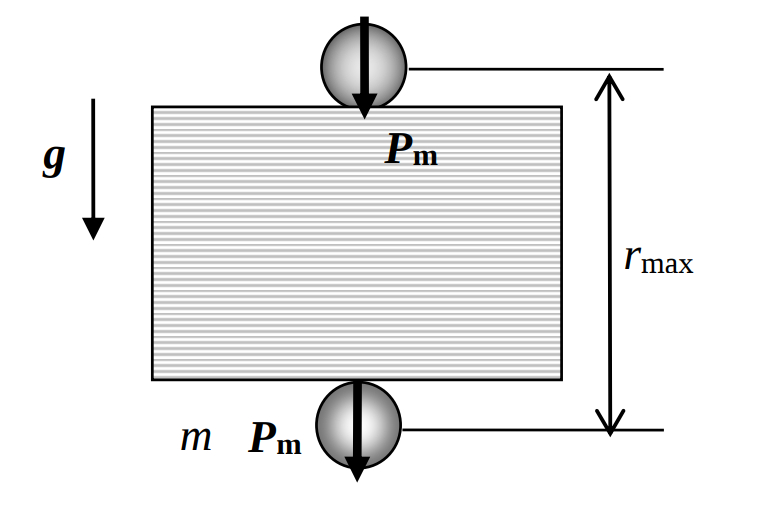
\includegraphics[width = 10cm]{1}}
	\caption{Определение магнитного момента шариков по силе тяжести}
	\label{fig:image}
\end{figure}

По величине магнитного момента $P_m$ можно рассчитать величину индукции магнитного поля вблизи любой точки на поверхности шара радиуса $R$. Максимальная величина индукции
наблюдаются на полюсах:
$$
	\vec{B_p} = 2\frac{\vec{P_m}}{R^3}
$$

\vspace{1cm}
\textbf{Определение величины магнитного момента по силе сцепления магнитных шариков (Метод B)}

Величину магнитного момента шариков можно определить также по силе их сцепления. Она определяется как сила, необходимая для разрыва двух сцепившихся магнитных шариков. Сила сцепления максимальна, если шары соединяются своими противоположными полюсами. Максимальную силу сцепления можно определить по весу магнитной цепочки, которую способен удержать самый верхний магнитный шарик. Если цепь состоит из одинаковых магнитных шариков (см. рис. 2, а), то при определённой длине она отрывается от верхнего шарика. При этом, учитывая, что сила притяжения убывает как $r$ в четвёртой степени ($r$ -- расстояния между центрами шаров) $F \sim 1/r$, для рассчёта прочности цепочки достаточно учитывать силу взаимодействия верхнего шара с тремя-четырьмя ближайшими соседями. 

\begin{figure}[h!]
	\center{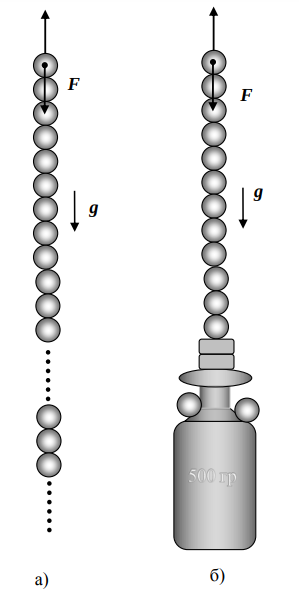
\includegraphics[width = 5cm]{2}}
	\caption{Определение магнитного момента шариков по силе сцепления}
	\label{fig:image}
\end{figure}

Если сила сцепления двух одинаковых шаров диаметром $d$ c магнитными моментами $P_m$ равна
$$
	F_0 = 6\frac{P_m^2}{d^4}
$$
то минимальный вес цепочки, при которой она оторвётся от верхнего шарика равен
$$
	F = 6\frac{P_m^2}{d^4} + 6\frac{P_m^2}{(2d)^4} + ... = F_0(1 + \frac{1}{2^4} + \frac{1}{3^4} + ...) \approx 1.08 F_0
$$
При вычислениях мы ограничились четырьмя членами ряда.

Таким образом, сила сцепления двух шаров равна
$$
	F = F_0\cdot1.08
$$
При этом совсем не обязательно составлять цепочку только из одинаковых шариков: на расстояниях, превышающих 20-30 диаметров шариков, можно подцепить всё, что примагничивается (см. рис. 2, б), -- на результат это практически не повлияет, в чем не сложно убедиться экспериментально.

\vspace{1cm}
\textbf{Измерение горизонтальной составляющей индукции магнитного поля Земли}

Магнитное поле Земли в настоящей работе определяется по периоду крутильных колебаний магнитной стрелки вокруг вертикальной оси. «Магнитная стрелка» образована из сцепленных друг с другом противоположными полюсами шариков и с помощью $\Lambda$-образного подвеса подвешена в горизонтальном положении (см. рис. 3). Магнитные моменты шариков направлены в одну сторону вдоль оси «стрелки». Под действием вращательного момента $\vec{M} = \vec{P_0}\times\vec{B}$ магнитный момент «стрелки» $\vec{P_0}$ выстроится вдоль горизонтальной составляющей магнитного поля Земли $\vec{B_h}$ в направлении $S \rightarrow N$. При отклонении «стрелки» на угол $\Theta$ от равновесного положения в горизонтальной плоскости возникают крутильные колебания вокруг вертикальной оси, проходящей через середину стрелки. Если пренебречь упругостью нити, то уравнение крутильных колебаний такого маятника определяется возвращающим моментом сил $M = -P_0B_h\sin\Theta$, действующим на «стрелку» со стороны магнитного поля Земли, и моментом инерции 
$I_n$ «стрелки» относительно оси вращения.

\begin{figure}[h!]
	\center{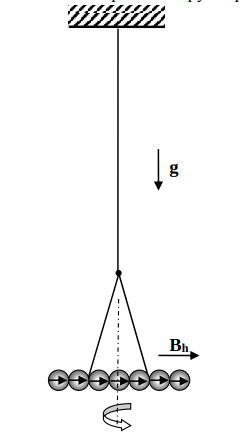
\includegraphics[width = 5cm]{3}}
	\caption{Крутильный маятник}
	\label{fig:image}
\end{figure}

При малых амплитудах ($\sin\Theta \approx \Theta$) уравнение колебаний «стрелки» имеет вид:
$$
	I_n\ddot{\Theta} + P_0B_h\Theta = 0
$$
Период колебаний
$$
	T = 2\pi\sqrt{\frac{I_n}{P_0B_h}} = 2\pi\sqrt{\frac{I_n}{nP_mB_h}}
$$
где $P_0 = nP_m$ -- полный магнитный момент магнитной «стрелки», составленной из $n$ шариков.

Момент инерции «стрелки», состоящей из $n$ шариков, как не сложно убедиться, с хорошей точностью равен моменту инерции тонкого однородного стержня массой $m_\text{ст} = nm$ и длиной $l_\text{ст} = nd$:
$$
	I_n = \frac{1}{12}m_\text{ст}l^2_\text{ст} = \frac{1}{12}nm(nd)^2 = \frac{1}{12}n^3md^2
$$

Даже для трёх шариков момент инерции, рассчитанный по приближённой формуле, отличается от точного результата примерно на 2\%, а для $n\geq 5$ -- различие не превышает процента; если же учесть, что $T \sim \sqrt{I_n}$, то для всех $n \geq 3$ погрешность наших расчетов для периода колебаний $T$ не превысит процента, что освобождает нас от необходимости вводить поправочные коэффициенты.

Таким образом, в нашем приближении период колебаний маятника оказывается пропорциональным числу шаров $n$, составляющих «стрелку»:
$$
	T(n) = 2\pi\sqrt{\frac{I_n}{nP_mB_h}} = \pi n\sqrt{\frac{md^2}{3P_mB_h}} = kn,
$$
где $k = \pi\sqrt{\frac{md^2}{3P_mB_h}}$.

При выводе этой формулы предполагалось, что магнитный момент -- величина аддитивная: полный магнитный момент системы магнитов («стрелки») равен векторной сумме магнитных моментов шариков, составляющих «стрелку». Экспериментальное подтверждение этой зависимости ($T \sim n$) будет являться косвенным доказательством наших предположений о магнитожёсткости материала магнитов и, соответственно, свойства аддитивности магнитных моментов шаров.

\vspace{1cm}
\textbf{Измерение вертикальной составляющей индукции магнитного поля Земли. Магнитное наклонение}

Для измерения вертикальной $B_v$ составляющей вектора индукции поля Земли используется та же установка, что и для измерения горизонтальной составляющей с тем лишь отличием,
что магнитная «стрелка» подвешивается на нити без $\Lambda$-образного подвеса. В этом случае магнитная «стрелка», составленная из чётного числа шариков и подвешенная на тонкой нити за середину, расположится не горизонтально, а под некоторым, отличным от нуля, углом к горизонту (см. рис. 4, а). Это связано с тем, что вектор $\vec{B}$ индукции магнитного поля Земли в общем случае не горизонтален, а образует с горизонтом угол $\beta$, зависящим от географической широты $\varphi$ места, где проводится опыт. Величина угла $\beta$ называется магнитным наклонением.

\begin{figure}[h!]
	\center{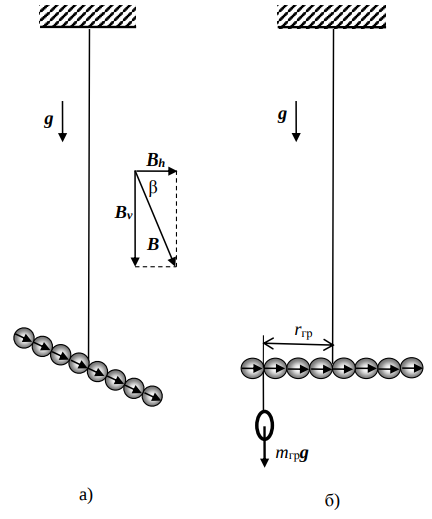
\includegraphics[width = 10cm]{4}}
	\caption{Измерение вертикальной составляющей индукции магнитного поля Земли}
	\label{fig:image}
\end{figure}

С помощью небольшого дополнительного грузика «стрелку» можно «выровнять», расположив её горизонтально (см. рис. 4, б): в этом случае момент силы тяжести груза относительно
точки подвеса будет равен моменту сил, действующих на «стрелку» со стороны магнитного поля Земли. Если масса уравновешивающего груза равна $m_\text{гр}$, плечо силы тяжести $r_\text{гр}$, а полный магнитный момент «стрелки» $P_0 = nP_m$, то в равновесии:
$$
	m_\text{гр}gr_\text{гр} = P_0B_v = nP_mB_v
$$

Видно, что момент $M(n)$ силы тяжести уравновешивающего груза пропорционален числу $n$ шариков, образующих магнитную «стрелку»:
$$
	M(n) = An,
$$
где $A = P_mB_v$.



\newpage
\textbf{Ход работы:}

1. Определение $P_m$ способом А.

Для начала взвесим несколько шариков. Для 12 шариков получим:
$$
	m_{12} = (5891 \pm 3)\cdot10^{-3} \text{г}
$$
откуда сразу вытекает:
$$
	m = (4910 \pm 3)\cdot10^{-4} \text{г}
$$

Измерим диаметр шарика:
$$
	d = (535 \pm 2)\cdot10^{-3} \text{см}
$$

Определим, на каком расстоянии сила магнитного взаимодействия перестает уравновешивать $mg$, вставив между двумя шариками пластинку из немагнитного материала и постепенно добавляя листы бумаги между ними. Получим
$$
	\Delta h = (1.77 \pm 0.02) \text{см}
$$

Теперь мы имеем достаточно данных, чтобы определить $P_m$:
$$
	P_m = \sqrt{\frac{mg(\Delta h + d)^4}{6}} = (48 \pm 2) \frac{\text{эрг}}{\text{Гс}}
$$
Погрешность определяем, считая $P_m = f(m, \Delta h, d)$.

Зная $d$, определим $V$ шарика:
$$
	V = \frac{4}{3}\pi\left(\frac{d}{2}\right)^3 = (80.1 \pm 0.3) \text{мм}^3
$$
и затем $p_m$:
$$
	p_m = \frac{P_m}{V} = (600 \pm 50) \frac{\text{эрг}}{\text{Гс}\cdot\text{см}^3}
$$


2. Определение $P_m$ методом В

Возьмем цепочку из шариков и будем добавлять к ней грузы. Получим:
$$
	m_1 = 304.7 \text{г}
$$
$$
	m_2 = 27.0 \text{г}
$$
Принимая массу шарика в качестве погрешности, получим:
$$
	m = m_1 + m_2 = (331.8 \pm 0.5) \text{г}
$$
Откуда:
$$
	F = \frac{mg}{1.08} = 3.015 \text{Н}
$$

$$
	P_m = \sqrt{\frac{F_0}{6}}d^2 = (65.3 \pm 0.2) \frac{\text{эрг}}{\text{Гс}}
$$

3. Определение горизонтальной составляющей магнитного поля Земли.

Снимем зависимость $10T(n)$:

\begin{center}
\begin{tabular}{|c|c|c|c|c|c|c|c|c|c|c|c|c|c|c|c|c|c|c|c|c|c|c|}
\hline
n		&	3		&	4		&	5		&	6		&	7		&	8		&	9		&	10		&	11		&	12		\\
\hline
10T,c	&	6.7		&	9.2		&	10.8	&	13.0	&	14.8	&	16.8	&	18.5	&	21.1	&	23.1	&	26.3	\\
\hline
\end{tabular}
\end{center}

Погрешности определения $n$ у нас нет, погрешность $10T$ примем равной 0.5с. 

\vspace{0.5cm}
\begin{tikzpicture}
\begin{axis}[
	ymin = 0,
	xmin = 0,
	height = 10cm,
	width  = 15cm,
	every axis y label/.style={at = {(ticklabel cs: 0.5)}, rotate = 90, anchor = near ticklabel},
	xlabel = {$n$},
	ylabel = {$T$, c},
	grid   = major
]
\addplot+[
	only marks,
	error bars/.cd, 
	y dir = both, y explicit,
	x dir = both, x explicit,
	]
coordinates{
	( 3, 0.67)	+-	(0, 0.05)
	( 4, 0.92)	+-	(0, 0.05)
	( 5, 1.08)	+-	(0, 0.05)
	( 6, 1.30)	+-	(0, 0.05)
	( 7, 1.48)	+-	(0, 0.05)
	( 8, 1.68)	+-	(0, 0.05)
	( 9, 1.85)	+-	(0, 0.05)
	(10, 2.11)	+-	(0, 0.05)
	(11, 2.31)	+-	(0, 0.05)
	(12, 2.63)	+-	(0, 0.05)
};

\addplot [mark = none]
coordinates{
	(0, 0)
	(12, 2.55647)
}; 

\end{axis}
\end{tikzpicture}

\vspace{1cm}
Из графика по МНК найдем угловой коэффициент $k$:
$$
	k = (0.21 \pm 0.01)c
$$
И определим $B_h$:
$$
	B_h = \frac{\pi^2md^2}{3k^2P_m} = (0.20 \pm 0.02) \text{Гс}
$$

4. Определение вертикальной составляющей магнитного поля Земли.

\begin{center}
\begin{tabular}{|c|c|c|c|c|c|c|c|c|c|c|c|c|c|c|c|c|c|}
\hline
n		&	$r_\text{гр}$, см	&	$m_\text{гр}, \text{кг}\cdot10^{-6}$	&	$M$, Нм$\cdot10^{-5}$	\\
\hline
12		&	2.68				&	133										&	3.49					\\
\hline
10		&	2.14				&	135										&	2.83					\\
\hline
8		&	1.61				&	118										&	1.86					\\
\hline
6		&	1.07				&	151										&	1.59					\\
\hline
4		&	0.54				&	175										&	0.92					\\
\hline
\end{tabular}
\end{center}

Погрешность оценим на глаз, как как измерения также проводились на глаз. Для оценки возьмем погрешность $\approx 10\% \approx 0.2 \text{Нм}\cdot10^{-5}$.

\vspace{0.5cm}
\begin{tikzpicture}
\begin{axis}[
	ymin = 0,
	xmin = 0,
	height = 10cm,
	width  = 15cm,
	every axis y label/.style={at = {(ticklabel cs: 0.5)}, rotate = 90, anchor = near ticklabel},
	xlabel = {$n$},
	ylabel = {$M$, Нм$\cdot10^{-5}$},
	grid   = major
]
\addplot+[
	only marks,
	error bars/.cd, 
	y dir = both, y explicit,
	x dir = both, x explicit,
	]
coordinates{
	( 4, 0.92)	+-	(0, 0.2)
	( 6, 1.59)	+-	(0, 0.2)
	( 8, 1.86)	+-	(0, 0.2)
	(10, 2.83)	+-	(0, 0.2)
	(12, 3.49)	+-	(0, 0.2)
};

\addplot [mark = none]
coordinates{
	(0, 0)
	(12, 3.276)
}; 

\end{axis}
\end{tikzpicture}

Из графика по МНК определим $A$:
$$
	A = 0.32 \text{Нм}\cdot10^{-5}
$$
Случайную погрешность $A$ получим из МНК:
$$
	\sigma_\text{случ} = 0.5 \text{Нм}\cdot10^{-5}
$$
Приборную возьмем равной $0.2 \text{Нм}\cdot10^{-5}$. В итоге получим:
$$
	A = (0.32 \pm 0.06) \text{Нм}\cdot10^{-5}
$$
Откуда несложно получить $B_v$:
$$
	B_v = \frac{A}{P_m} = (65 \pm 13)\cdot10^{-2} \text{Гс}
$$

5. Определение магнитного наклонения.

По определению:
$$
	\beta = \arctg\frac{B_v}{B_h} = (73 \pm 14)^\circ
$$
Также определим значение $B$:
$$
	B = \sqrt{B_v^2 + B_h^2} = (0.68 \pm 0.17) \text{Гс}
$$

\newpage
В данной лаборатороной работе мы определили характеристики шарообразных неодимовых магнитов и, используя законы взаимодействия магнитных моментов с полем, измерить горизонтальную и вертикальную составляющие индукции магнитного поля Земли и магнитное наклонение в Долгопрудном.


\end{document}